\documentclass{article}

% Packages required to support encoding
\usepackage{ucs}
\usepackage[utf8x]{inputenc}

% Packages required by code


% Packages always used
\usepackage{graphicx}
\usepackage{hyperref}
\usepackage{xspace}
\usepackage[usenames,dvipsnames]{color}
\hypersetup{colorlinks=true,urlcolor=blue}

\usepackage{changepage}
%\usepackage{accents}
\def\utilde#1{\mathord{\vtop{\ialign{##\crcr
$\hfil\displaystyle{#1}\hfil$\crcr\noalign{\kern1.5pt\nointerlineskip}
$\hfil\tilde{}\hfil$\crcr\noalign{\kern1.5pt}}}}}

\usepackage{geometry}
\geometry{letterpaper,textwidth=350pt,textheight=680pt,tmargin=60pt,
            left=72pt,footskip=24pt,headsep=18pt,headheight=14pt}
\usepackage{amsmath}
\usepackage{amssymb}
\usepackage{textcase}
\usepackage{soul}

%% THINGS KYLE HAS ADDED
\newcommand{\lp}{\left(}
\newcommand{\rp}{\right)}
\newcommand{\inv}{^{-1}}
\newcommand{\mynt}{ {\color{red} Note:} }
\newcommand{\myans}{{\color{blue}\textbf{Answer}}\newline}
\DeclareMathOperator{\rank}{rank}

%%


\newcommand{\mat}[1]{\boldsymbol{#1}}
\renewcommand{\vec}[1]{\boldsymbol{\mathrm{#1}}}
\newcommand{\vecalt}[1]{\boldsymbol{#1}}

\newcommand{\conj}[1]{\overline{#1}}

\newcommand{\normof}[1]{\|#1\|}
\newcommand{\onormof}[2]{\|#1\|_{#2}}

\newcommand{\itr}[2]{#1^{(#2)}}
\newcommand{\itn}[1]{^{(#1)}}

\newcommand{\eps}{\varepsilon}
\newcommand{\kron}{\otimes}

\DeclareMathOperator{\diag}{diag}
\DeclareMathOperator{\trace}{trace}
\DeclareMathOperator{\tvec}{vec}

\newcommand{\prob}{\mathbb{P}}
\newcommand{\probof}[1]{\prob\left\{ #1 \right\}}

\newcommand{\pmat}[1]{\begin{pmatrix} #1 \end{pmatrix}}
\newcommand{\bmat}[1]{\begin{bmatrix} #1 \end{bmatrix}}
\newcommand{\spmat}[1]{\left(\begin{smallmatrix} #1 \end{smallmatrix}\right)}
\newcommand{\sbmat}[1]{\left[\begin{smallmatrix} #1 \end{smallmatrix}\right]}

\newcommand{\RR}{\mathbb{R}}
\newcommand{\CC}{\mathbb{C}}

\providecommand{\eye}{\mat{I}}
\providecommand{\mA}{\ensuremath{\mat{A}}}
\providecommand{\mB}{\ensuremath{\mat{B}}}
\providecommand{\mC}{\ensuremath{\mat{C}}}
\providecommand{\mD}{\ensuremath{\mat{D}}}
\providecommand{\mE}{\ensuremath{\mat{E}}}
\providecommand{\mF}{\ensuremath{\mat{F}}}
\providecommand{\mG}{\ensuremath{\mat{G}}}
\providecommand{\mH}{\ensuremath{\mat{H}}}
\providecommand{\mI}{\ensuremath{\mat{I}}}
\providecommand{\mJ}{\ensuremath{\mat{J}}}
\providecommand{\mK}{\ensuremath{\mat{K}}}
\providecommand{\mL}{\ensuremath{\mat{L}}}
\providecommand{\mM}{\ensuremath{\mat{M}}}
\providecommand{\mN}{\ensuremath{\mat{N}}}
\providecommand{\mO}{\ensuremath{\mat{O}}}
\providecommand{\mP}{\ensuremath{\mat{P}}}
\providecommand{\mQ}{\ensuremath{\mat{Q}}}
\providecommand{\mR}{\ensuremath{\mat{R}}}
\providecommand{\mS}{\ensuremath{\mat{S}}}
\providecommand{\mT}{\ensuremath{\mat{T}}}
\providecommand{\mU}{\ensuremath{\mat{U}}}
\providecommand{\mV}{\ensuremath{\mat{V}}}
\providecommand{\mW}{\ensuremath{\mat{W}}}
\providecommand{\mX}{\ensuremath{\mat{X}}}
\providecommand{\mY}{\ensuremath{\mat{Y}}}
\providecommand{\mZ}{\ensuremath{\mat{Z}}}
\providecommand{\mLambda}{\ensuremath{\mat{\Lambda}}}
\providecommand{\mPbar}{\bar{\mP}}

\providecommand{\ones}{\vec{e}}
\providecommand{\va}{\ensuremath{\vec{a}}}
\providecommand{\vb}{\ensuremath{\vec{b}}}
\providecommand{\vc}{\ensuremath{\vec{c}}}
\providecommand{\vd}{\ensuremath{\vec{d}}}
\providecommand{\ve}{\ensuremath{\vec{e}}}
\providecommand{\vf}{\ensuremath{\vec{f}}}
\providecommand{\vg}{\ensuremath{\vec{g}}}
\providecommand{\vh}{\ensuremath{\vec{h}}}
\providecommand{\vi}{\ensuremath{\vec{i}}}
\providecommand{\vj}{\ensuremath{\vec{j}}}
\providecommand{\vk}{\ensuremath{\vec{k}}}
\providecommand{\vl}{\ensuremath{\vec{l}}}
\providecommand{\vm}{\ensuremath{\vec{l}}}
\providecommand{\vn}{\ensuremath{\vec{n}}}
\providecommand{\vo}{\ensuremath{\vec{o}}}
\providecommand{\vp}{\ensuremath{\vec{p}}}
\providecommand{\vq}{\ensuremath{\vec{q}}}
\providecommand{\vr}{\ensuremath{\vec{r}}}
\providecommand{\vs}{\ensuremath{\vec{s}}}
\providecommand{\vt}{\ensuremath{\vec{t}}}
\providecommand{\vu}{\ensuremath{\vec{u}}}
\providecommand{\vv}{\ensuremath{\vec{v}}}
\providecommand{\vw}{\ensuremath{\vec{w}}}
\providecommand{\vx}{\ensuremath{\vec{x}}}
\providecommand{\vy}{\ensuremath{\vec{y}}}
\providecommand{\vz}{\ensuremath{\vec{z}}}
\providecommand{\vpi}{\ensuremath{\vecalt{\pi}}}

\sodef\allcapsspacing{\upshape}{0.15em}{0.65em}{0.6em}%

\makeatletter
\def\maketitle{%
\par
\hrule height 0.75pt\vspace{1ex}
\par\noindent
\begin{minipage}{0.5\textwidth}
\scshape
purdue university  \\

\end{minipage}
\begin{minipage}{0.5\textwidth}
\raggedleft
\MakeTextUppercase{\allcapsspacing{\@title}}\\[0.2ex]
\textit{\@author}\\[0.2ex]
\textit{\@date}
\end{minipage}
\par\vspace{1ex}
\hrule height 1pt
\vspace{2ex}
\par
}
\makeatother

\author{Shuvra Kanti Nath}
\title{RNA-Seq Documentation}
% auto generate a title
\AtBeginDocument{\maketitle}



\begin{document} 
Summary: This document shows the steps in details to generate read count data from gtf files for a genome.\newline
Machine: Carter \newline
Softwares needed: Flux Simulator, samtools, bowtie, tophat \newline
Data in : /scratch/carter/n/naths \newline
Steps for Human Genome processing:\newline
\begin{description}
  \item[Step 1(Get Genome Data)]\hfill \\
  First download the  chromFa.tar.gz from  \url{http://hgdownload.soe.ucsc.edu/goldenPath/hg19/bigZips/} and untar it. \newline  

  \item[Step 2(Run Flux Simulator)] \hfill \\
Run:\newline
/homes/naths/flux-simulator-1.2.1/bin/flux-simulator -p hg19.par . \newline
If successful, a .fasta file will be generated. See the hg19.par bellow.

\begin{verbatim}
## File locations
REF_FILE_NAME   chr1_refseq_sub.gtf
GEN_DIR         genomes/


## Expression
NB_MOLECULES    20000
TSS_MEAN	NaN
POLYA_SCALE     NaN
POLYA_SHAPE     NaN
EXPRESSION_K	-0.9

## Fragmentation
FRAG_SUBSTRATE  RNA
FRAG_METHOD     UR

## RT parameters
RTRANSCRIPTION YES
RT_MOTIF       default
RT_PRIMER      RH
RT_LOSSLESS    YES
RT_MIN         500
RT_MAX         5500

## PCR / Filtering
PCR_DISTRIBUTION  default
FILTERING         YES
SIZE_SAMPLING     AC
SIZE_DISTRIBUTION N(200,25)

# Amplifcation
GC_MEAN	NaN

# Sequencing
READ_NUMBER     20000
READ_LENGTH     50
PAIRED_END      YES
FASTA           YES
UNIQUE_IDS	YES
\end{verbatim}


  \item[Step 3(Download gtf file)]  \hfill \\
Download .gtf file from \url{https://genome.ucsc.edu/cgi-bin/hgTables}. Use( clade: mammal, genome:human, assembly: hg19, track: refseq genes, table: refgene, output format : gtf file format).
The file should look like Figure ~\ref{fig:refgene}.

\begin{figure}[htpb]
\begin{center} 
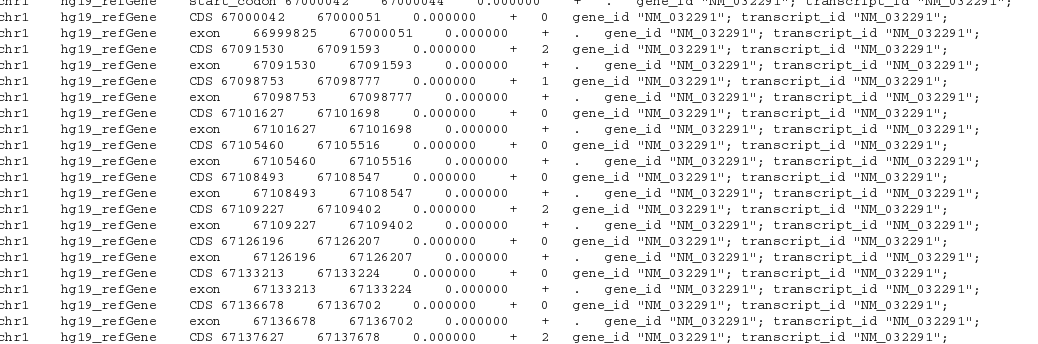
\includegraphics[scale=0.4]{refgene.png}
\end{center}
\caption{ gtf file}
\label{fig:refgene}
\end{figure}


  \item[Step 4(Choose a subset from the gtf)]  \hfill \\
The downloaded gtf file is very big and will take a very long processing time. So, we want a subset of gtf file corresponding to few genes and their isoforms. From \url{https://genome.ucsc.edu/cgi-bin/hgTables}, select group: all tables, table: refFlat, output format: all fields from selected table.
The selected table will look like:
Figure ~\ref{fig:isoform}.

\begin{figure}[htpb]
\begin{center} 
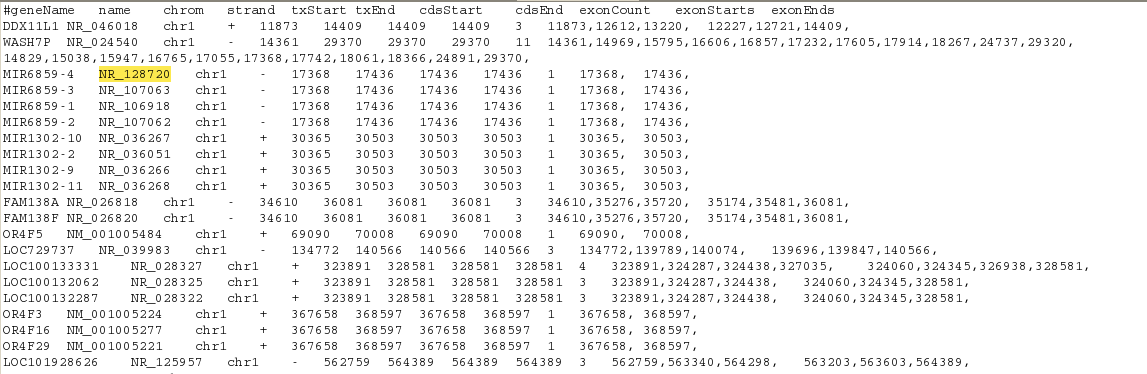
\includegraphics[scale=0.4]{isoform.png}
\end{center}
\caption{ gene and isoform table}
\label{fig:isoform}
\end{figure}
\#geneName and name show the name of gene and corresponding isoform names. Now you can choose any genes and the corresponding isoforms that you want to process. In a list.txt file write down the isoform names like:
\begin{verbatim}
NM_021170
NM_001142467
NR_047526
\end{verbatim}
To get a subest of gtf file corresponding to this isoforms, run:
\begin{verbatim}
grep -f list.txt hg19.gtf > subset.gtf
\end{verbatim}

Example: \newline
From the genes of chr1:
LINC01128 , LOC100130417, LOC100133331, PERM1, HES4\newline
I chose the isoforms: 
\begin{verbatim}
NM_021170,
NM_001142467,
NR_047526,
NR_047525,
NR_047524,
NR_047523,
NR_047521,
NR_047519,
NR_122045,
NR_026874,
NR_028327,
NM_001291366,
NM_001291367,
NR_028327
\end{verbatim}

\item[Step 5 (Download Bowtie indices)] \hfill \\
Download pre-built bowtie indices from \url{http://bowtie-bio.sourceforge.net/manual.shtml}. \newline
Now run : \begin{verbatim} ./make_hg19.sh \end{verbatim} If it does not work, then run : bowtie2-build chr1.fa ..... chr17.fa hg19 \newline
This step will generate 4 files: hg19.1.bt2, hg19.2.bt2, hg19.3.bt2, hg19.4.bt2 .

\item[Step 6 (Run Tophat)] \hfill \\
Load tophat:

module use /apps/group/bioinformatics/modules \newline
module load tophat \newline
module load bowtie2 \newline
Run tophat: \newline
\begin{verbatim} 
tophat hg19 hg19.fasta (if single end read) 
tophat hg19 hg19_1.fasta hg19_2.fasta (if paired-end read)
\end{verbatim}

If successful, this will generate accepted\_hits.bam in tophat\_out folder.

\textbf{***}If you want to simulate single end reads, you need to specify "PARIED\_END NO" in the .par file while running flux-simulator.
If you had used paired-end reads, then .fasta generated from flux-simulator needed to be seperated into 2 files.\newline
Command:
\begin{verbatim} 
grep 'c.*/1' -A 1 hg19.fasta | sed '/--/d' > hg19_1.fasta
grep 'c.*/2' -A 1 hg19.fasta | sed '/--/d' > hg19_2.fasta
 \end{verbatim}

\item[Step 7 (Get the sam file)] \hfill \\
Run:
\begin{verbatim} 
module load samtools
samtools view -f 67 accepted_hits.bam | awk '$3=="chr1" {print $1,$2,$4,$6,$8,$9}' > sam
\end{verbatim}
You can use use flag 67 or 131. To know about the details about the flags go here: \url{http://broadinstitute.github.io/picard/explain-flags.html}.
The sam file(this was from paired-end) should look like : 
Figure ~\ref{fig:sam}.

\begin{figure}[htpb]
\begin{center} 
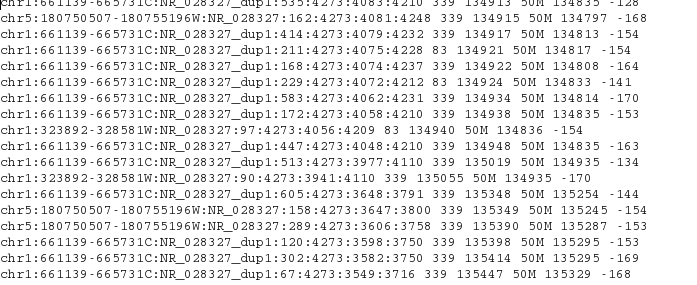
\includegraphics[scale=0.4]{sam.png}
\end{center}
\caption{ Sam file}
\label{fig:sam}
\end{figure}

\item[Step 8 (Generate read count)] \hfill \\

In case of paired-end reads,
Use the samtools to filter out the first mate and second mate separately. (All the reads and the mapping information are in the .bam file, but you need to separate them out)

\begin{verbatim} 
 samtools view -f 67 accepted_hits.bam | awk '{print $1,$2,$4,$6,$8,$9}' > sim_11.txt
 samtools view -f 97 accepted_hits.bam | awk '{print $1,$2,$4,$6,$8,$9}' > sim_12.txt
 
samtools view -f 131 accepted_hits.bam | awk '{print $1,$2,$4,$6,$8,$9}' > sim_21.txt
samtools view -f 145 accepted_hits.bam | awk '{print $1,$2,$4,$6,$8,$9}' > sim_22.txt


cat sim_11.txt sim_12.txt  > sim_1.txt
cat sim_21.txt sim_22.txt > sim_2.txt
\end{verbatim}

67, 97, 131 and 145 are different kinds of reads and may not be available in every study.

We have a .R script which takes the sam files sim\_1.txt, sim\_2.txt as input and generates the read count file.

\end{description}





\end{document}
